\section{Aufbau der WordClock}
Nach der mechanischen und elektrischen Vorbereitung, der Konstruktion sowie dem additiven \gls{3ddruck} der Bauteile, erfolgt die Montage des Gesamtsystems.  
Zunächst werden die \gls{led}-Streifen zugeschnitten und entsprechend der geplanten Anordnung auf die Grundplatte geklebt.
Hierzu wird das Layout auf die Grundplatte gezeichnet und die Positionen der \gls{led}s mit dem zugehörigen Buchstaben bzw. Symbol und den Indizes der \gls{led} beschriftet.
Dadurch kann überprüft werden, ob die korrekten Wörter angezeigt werden und die korrekte \gls{led} angesprochen wird.  
Anschließend werden die einzelnen Streifen durch Lötverbindungen verbunden (vgl. Abb~\ref{fig:VerlötetStreifen}).  
Die Anschlusskabel werden auf die Rückseite geführt.
Für den \gls{led}-Strang der Sekundenazeige werden vier weitere Bauteile gedruckt, um die \gls{led}-Bänder um die Kurve zu führen.
Diese sind fest auf der Grundplatte montiert und in Abb.~\ref{fig:VerlötetStreifen} zu sehen.
\begin{figure}[H]
	\centering
	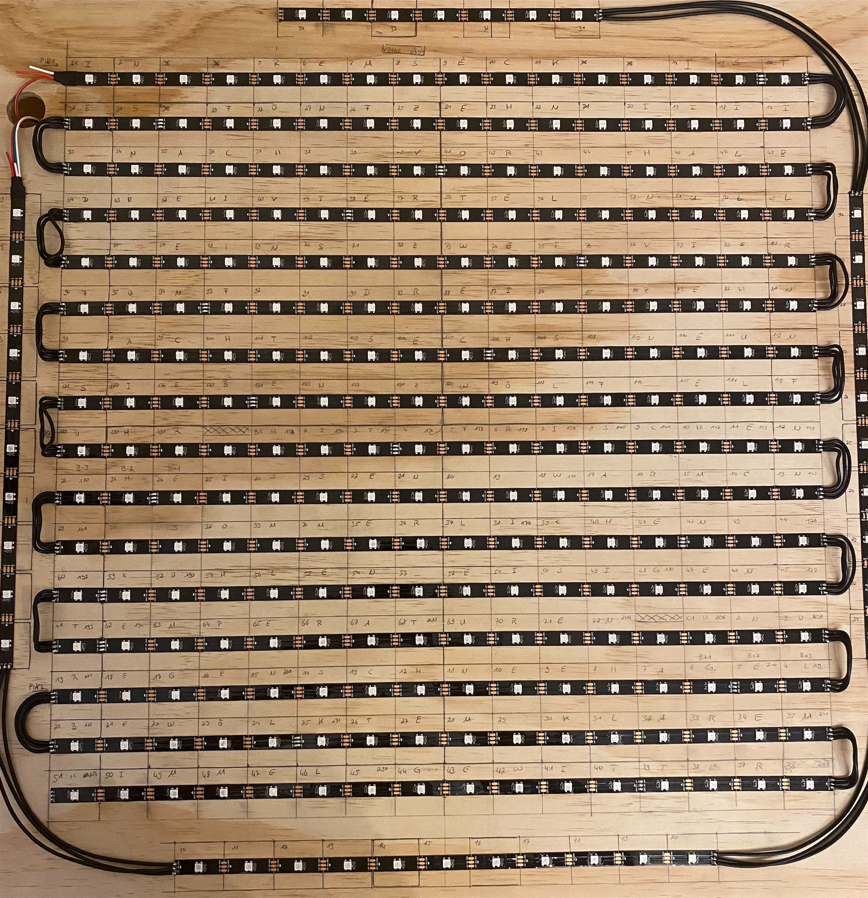
\includegraphics[width=0.60\linewidth]{inhalt/bilder/LEDsVerloetet.png}
	\caption[Installation aller \gls{led}-Stränge]{Grundplatte während der installation und dem verlöten der einzelnen \gls{led}-Streifen zu den drei \gls{led}-Strängen. In den Ecken der Grundplatte befinden sich die Bauteile, mit denen die \gls{led}-Bänder um die Kurve geführt werden.}
	\label{fig:VerlötetStreifen}
\end{figure}
Die Verbindung der Frontplatte zur Grundplatte erfolgt über die Eckteile.  
Hierzu werden Gewindeeinsätze, sogenannte Heatinsert, eingesetzt, die in das 3D-gedruckte Material integriert werden.
Die Heatinserts werden mit einem Lötkolben erhitzt und dann eingepresst (vgl. Abb.~\ref{fig:Heatinserts}).
\begin{figure}[H]
	\centering
	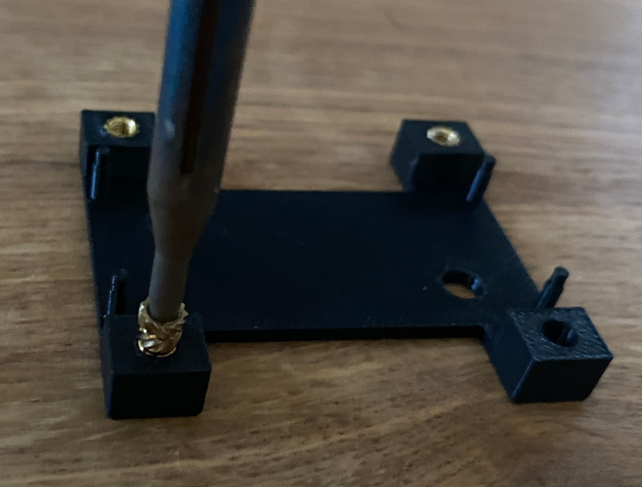
\includegraphics[width=0.4\linewidth]{inhalt/bilder/BeispielHeatinsertESPHalter.png}
	\caption[Einpressvorgang der Heatinserts]{Einpressvorgang der Heatinserts am Beispiel des \gls{esp32c6}-Halters.}
	\label{fig:Heatinserts}
\end{figure}  
Die Befestigung erfolgt anschließend mit M4x20-Schrauben.  
Die Verbindung der einzelnen Frontplattenbauteile untereinander, erfolgt über Durchgangsbohrungen.  
Hierbei werden M3x12-Schrauben in Kombination mit Muttern und Unterlegscheiben verwendet.
Weiterhin werden die Halterung für den \gls{esp32c6}, die Halterung für die Hohlsteckerbuchse, die Halterung für den \gls{dht22} sowie die Abstandshalter und Befestigungspunkte auf der Rückseite der Grundplatte verschraubt.

Für die initiale Inbetriebnahme und Implementierung der Software wird der Mikrocontroller provisorisch angeschlossen.  
Hierzu werden Jumperkabel und Klemmen verwendet. 
Es wird je eine Klemme als Sternpunkt für Ground und +5~V verwendet und zusätzlich je eine Klemme pro Signalleitung.
Es gibt drei dreipolige Steckverbinder mit je einem Ground-Anschluss, einem +5~V-Anschluss und einem Signal-Anschluss (vgl. Abb.~\ref{fig:TischIBN}).
An den \gls{led}-Strängen der WordClock ist das jeweilige Gegenstück der Steckverbinder angebracht. 
Diese Vorgehensweise ermöglicht eine flexible Anpassung der Verdrahtung und ein schnelles trennen und wieder verbinden der einzelnen Stränge während der Test- und Evaluationsphase.

\begin{figure}[H]
	\centering
	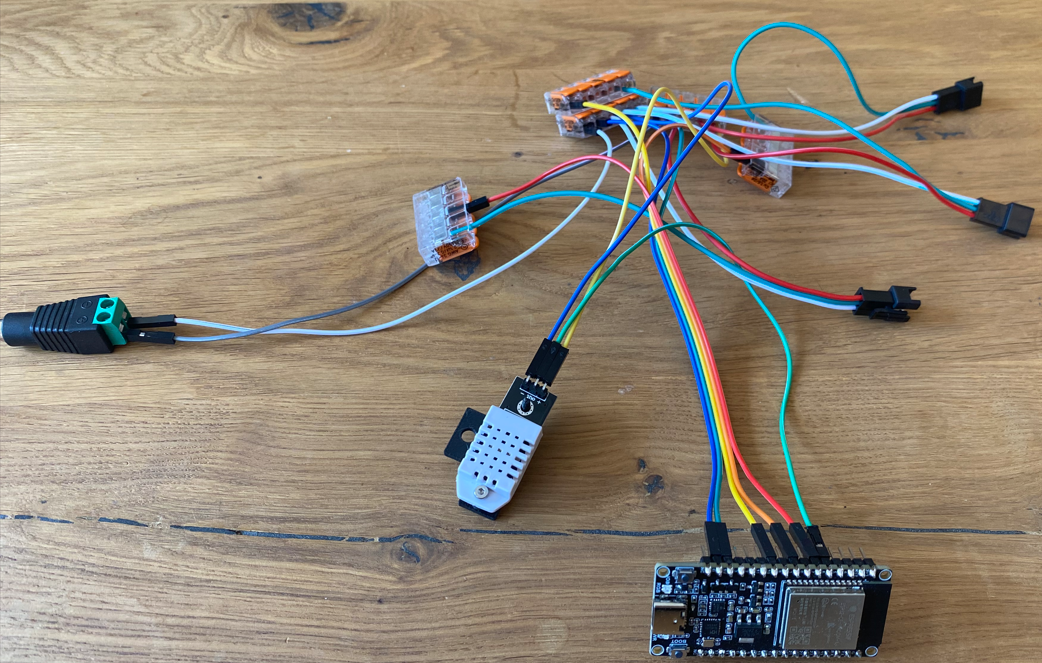
\includegraphics[width=0.8\linewidth]{inhalt/bilder/Jumperkabelaufbau.png}
	\caption[Der für die Inbetriebnahme verwendete elektrische Aufbau]{Der für die Inbetriebnahme verwendete elektrische Aufbau und der Anschluss des Mikrocontroller, welcher zunächst aus Jumperkabeln, Klemmen und dreipoligen Steckverbindern besteht.}
	\label{fig:TischIBN}
\end{figure}